%%
%% N.~13 (ex N.~18):
%% Anstreichungen und Anmerkungen in Pierre Le Cazre, Physica demonstratio
%% PR: Stand 12.04.2016
%%
\begin{ledgroupsized}[r]{120mm}
\footnotesize 
\pstart 
\noindent\textbf{\"{U}berlieferung:}
\pend
\end{ledgroupsized}  
\begin{ledgroupsized}[r]{114mm}
\footnotesize 
\pstart \parindent -6mm
\makebox[6mm][l]{\textit{LiH}}%
Anstreichungen und Anmerkungen in
\textsc{P. Le Cazre},\cite{01022} \textit{Physica demonstratio qua \mbox{ratio}, men\-sura, modus ac potentia accelerationis motus in naturali descensu gravium deter\-mi\-nan\-tur}, Paris 1645:
\textsc{Hannover}, GWLB, Leibn. Marg. 126. Textverlust durch Beschnei\-dung der Ränder.
\pend
\end{ledgroupsized}
% \normalsize
\vspace*{5mm}
%
\begin{ledgroup}
\footnotesize 
\pstart
\noindent\footnotesize{\textbf{Datierungsgr\"{u}nde:}
Hinweise auf die Thematik der \textit{Physica demonstratio} finden sich in N.~1, %?? = Aus und zu Gassendi
N.~7 %?? = Aus und zu Pardis, Statique
und N.~10, %?? = De vitandis erroibus geometricis
Anspielungen in N.~34\textsubscript{4} % = R/5.4: Essai de quelques démonstrations géometriques du frottement
und N.~36. %?? = LH35,9,11 Bl. 1-2 + LH35,9,11 Bl. 3-4 = R/7: Du Frottment. Essais géometriques en fait de mécanique
Leibniz' Randbemerkungen dürften somit in einem Zeitraum vom Sommer 1672 bis zum Ende 1675 entstanden sein.
Die inhaltliche Verwandschaft mit den Stücken N.~14 %?? = LH37,05_130: De acceleratione
und N.~15 % = LH37,05_128-129: De motu gravium naturali
legt allerdings eine gemeinsame Datierung auf September 1672 bis März 1673 nahe.}
\pend
\end{ledgroup}
\count\Afootins=1200
\vspace*{8mm}
\count\Afootins=1200
\pstart 
\normalsize
\noindent
%\begin{wrapfigure}[12]{l}{0.20\textwidth}%0.1
%\vspace{-4mm}\centering%
%\hspace*{7mm}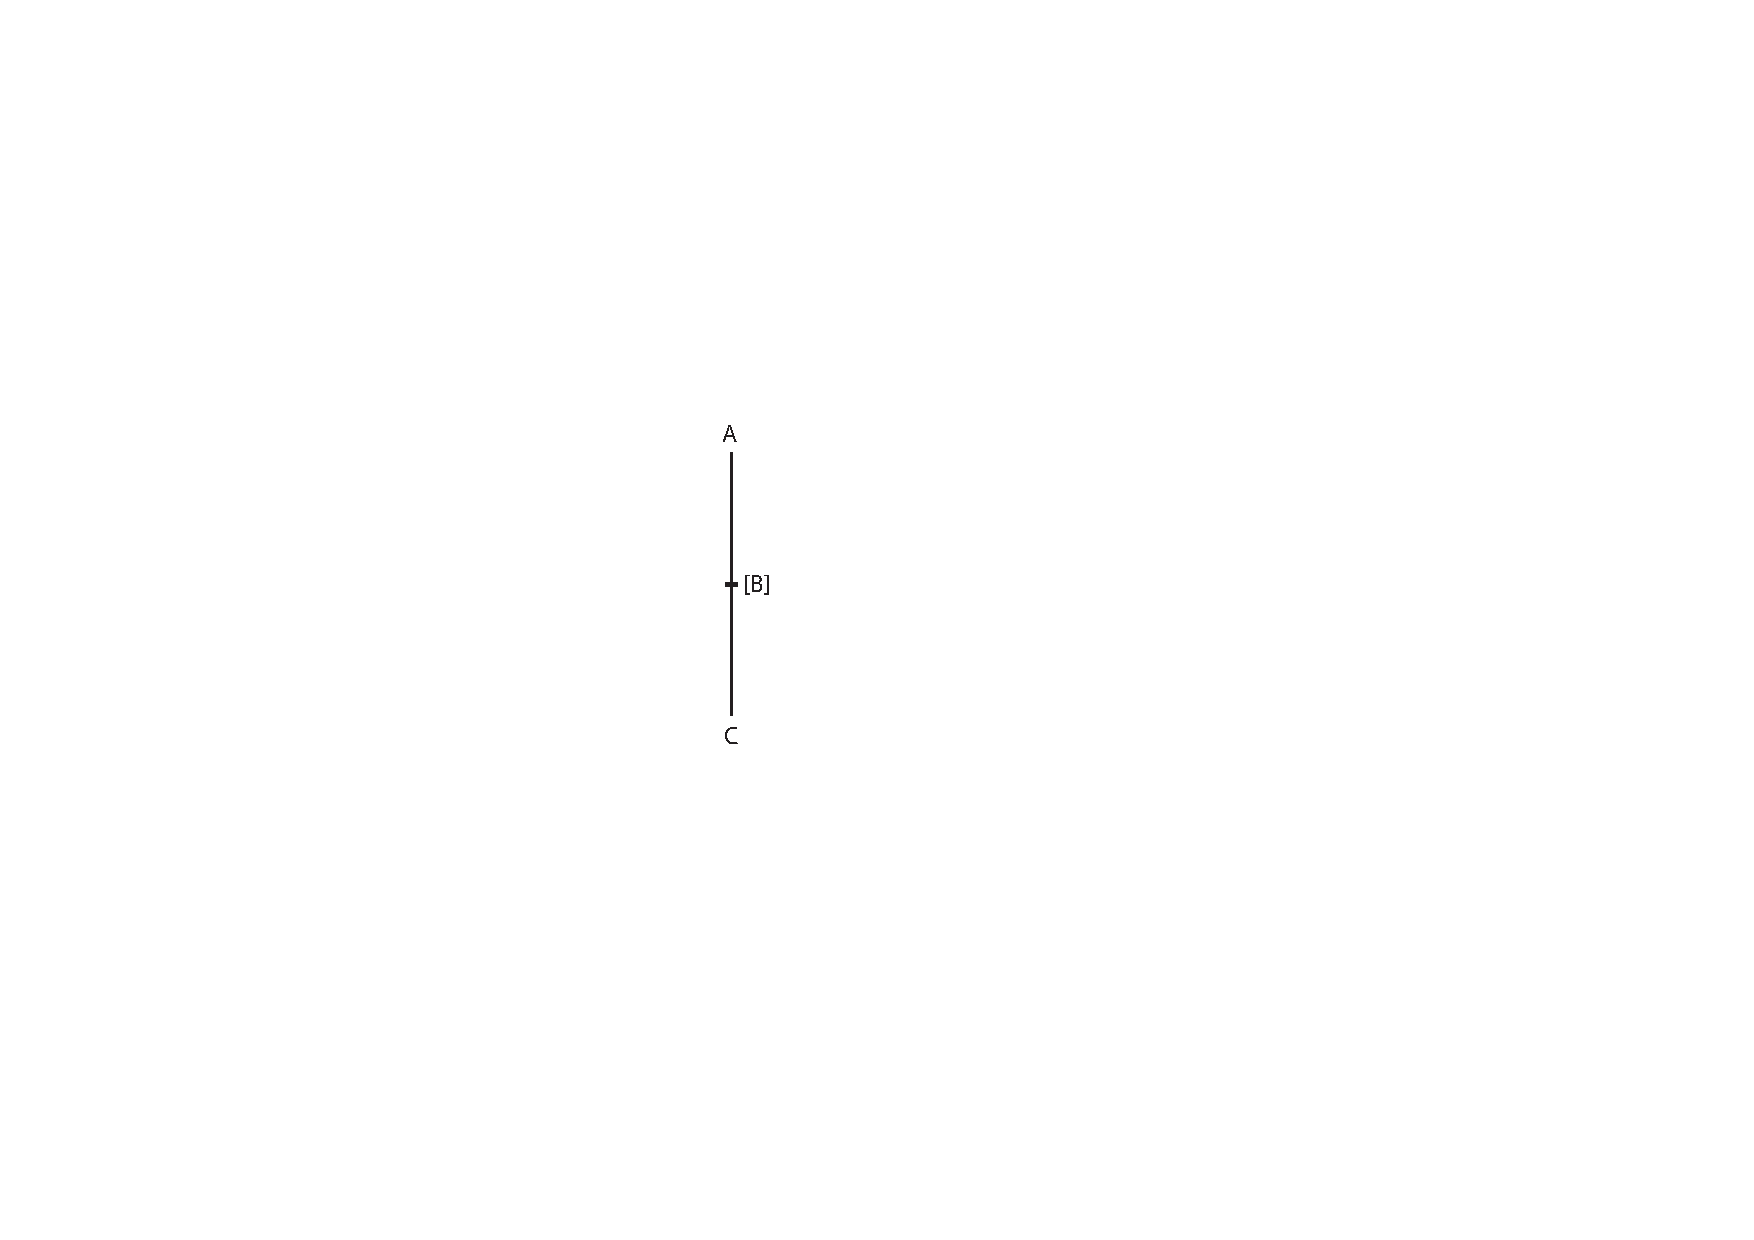
\includegraphics[trim = 1mm 1mm -13mm 2mm, clip, width=0.15\textwidth]{images/cazreus1645-d1.pdf}%-8mm
%\newline
%\noindent\centering
%[\textit{Fig. 1}]%
%\end{wrapfigure}
%\noindent%
[p. 8]
\textit{Si acceleratio\protect\index{Sachverzeichnis}{acceleratio} motus}
(inquit)
\textit{in descensu\protect\index{Sachverzeichnis}{descensus} grauium\protect\index{Sachverzeichnis}{grave},
aequalibus spatiis aequalia sumeret velocitatis incrementa, essent sine dubio velocitates %
%%
\edtext{}{\lemma{}\Afootnote{\textit{An} velocitates \textit{angeschlossen:} sub finem emensi spatii acquisitae\vspace{1.6mm}}
%%
inter se vt emensa spatia. At quotiescumque velocitates}
inter se sunt vt emensa spatia, debent necessario ea spatia, aut eodem, aut aequali tempore
%%
\edtext{percurri.}{\lemma{}\Afootnote{\textit{An} percurri \textit{angeschlossen:}
Negatur. Neque enim velocitates sub motus finem acquisitae,\textsuperscript{[a]} 
spatiis proportionales faciunt tempus aequale sed velocitates quibus tota spatia percursa sunt.
Est ergo verissimum ratiocinationi Galilaei\protect\index{Namensregister}{\textso{Galilei} (Galilaeus, Galileus), Galileo 1564-1642} inesse paralogismum.
Quanquam Cazraeus\protect\index{Namensregister}{\textso{Le Cazre} (Cazreus), Pierre 1589-1664} non videatur eum satis retexisse.%
\vspace*{2mm}%
\newline\footnotesize%
\textsuperscript{[a]} acquisitae, \textit{(1)}\ restari \textit{(2)}\ spatiis \textit{L}}}
%%
Si igitur velocitas acquisita per totam AC, eam rationem\hfill habeat\hfill ad\hfill velocitatem\hfill acquisitam\hfill per\hfill AB,\hfill
quam\hfill spatium\hfill AC,\hfill ad\hfill spatium\hfill AB,}
\pend
\newpage
\pstart
\noindent
\begin{wrapfigure}[12]{l}{0.20\textwidth}%0.1
\vspace{-4mm}\centering%
\hspace*{7mm}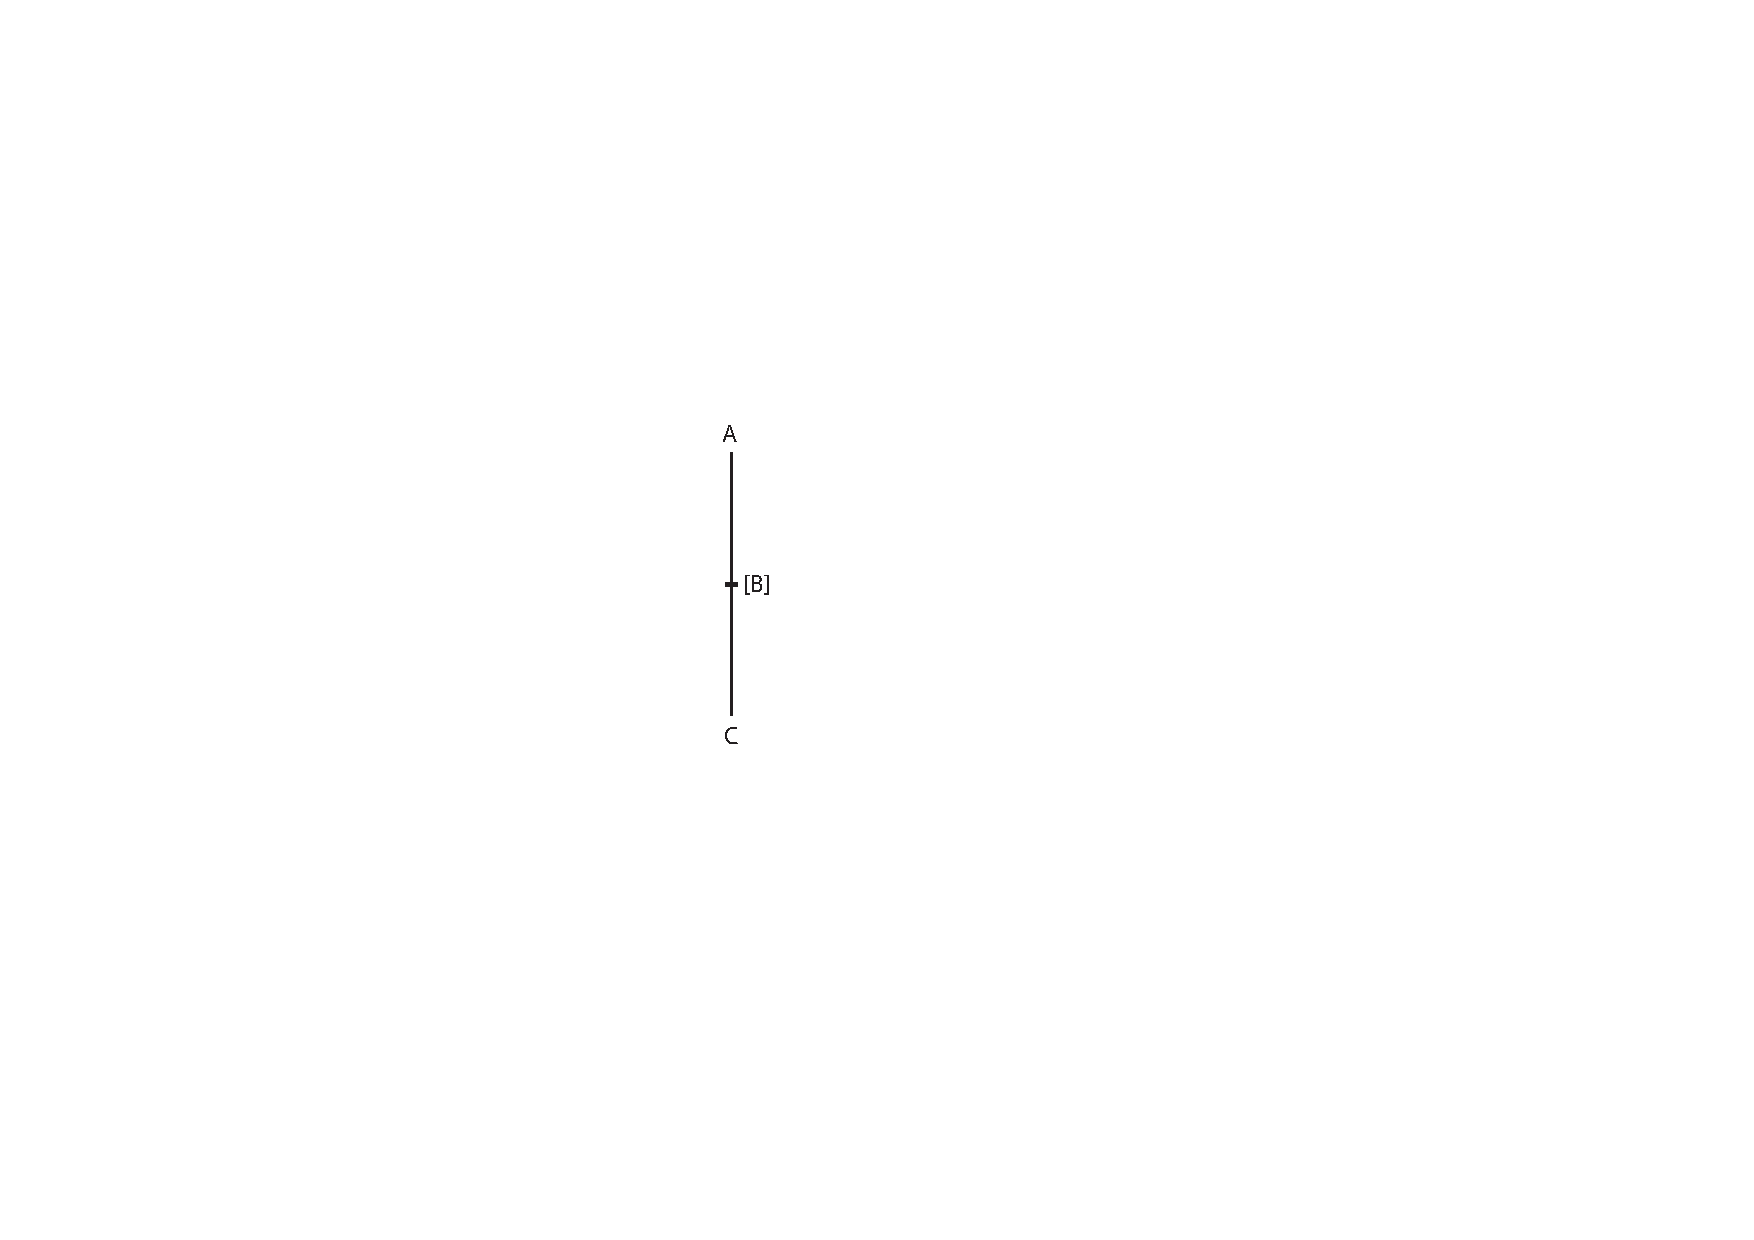
\includegraphics[trim = 1mm 1mm -13mm 2mm, clip, width=0.15\textwidth]{images/cazreus1645-d1.pdf}%-8mm
\newline
\noindent\centering
[\textit{Fig. 1}]%
\end{wrapfigure}
\noindent%
\textit{necesse est vt spatium totum AC, eodem, aut aequali tempore decurratur,
quo spatium AB absoluitur. Impossibile est autem vt corpus graue descendens per AC, eodem aut aequali tempore percurrat totam AC,
quo percurrit partem eius AB, nisi motus fiat in instanti.
Tam impossibile est igitur, vt velocitates in descensu\protect\index{Sachverzeichnis}{descensus}
grauium\protect\index{Sachverzeichnis}{grave} inter se sint vt emensa spatia,
(ac proinde vt etiam aequalibus spatiis crescant aequaliter) quam impossibile est motum illum fieri \edtext{in instanti.%
}{\lemma{\textit{in instanti}}\Cfootnote{\cite{00050}\textsc{G. Galilei}, \textit{Discorsi}, Leiden 1638, S.~164f. (\cite{00048}\textit{GO} VIII, S.~203f).
Das Zitat ist eine lateini\-sche Zusammenfassung von Galileis Argument.}}}
\pend
\count\Afootins=1200
% \newpage
\vspace*{8em}%
\pstart%
\noindent%
[p. 11]
[\textit{Gedruckte Marginalie zu Fig. 2}]
Experientia qua Galilaeus\protect\index{Namensregister}{\textso{Galilei} (Galilaeus, Galileus), Galileo 1564-1642}
suum Postulatum confirmare nititur.%
\edtext{}{\lemma{\hspace*{1,8mm}[\textit{Fig. 2}]}\killnumber\Afootnote{\textit{Zum Diagramm:}
\textit{K.H.D.} debent esse in eadem recta horizonti parallela.}}
\pend
\vspace*{0.5em}%
\begin{center}
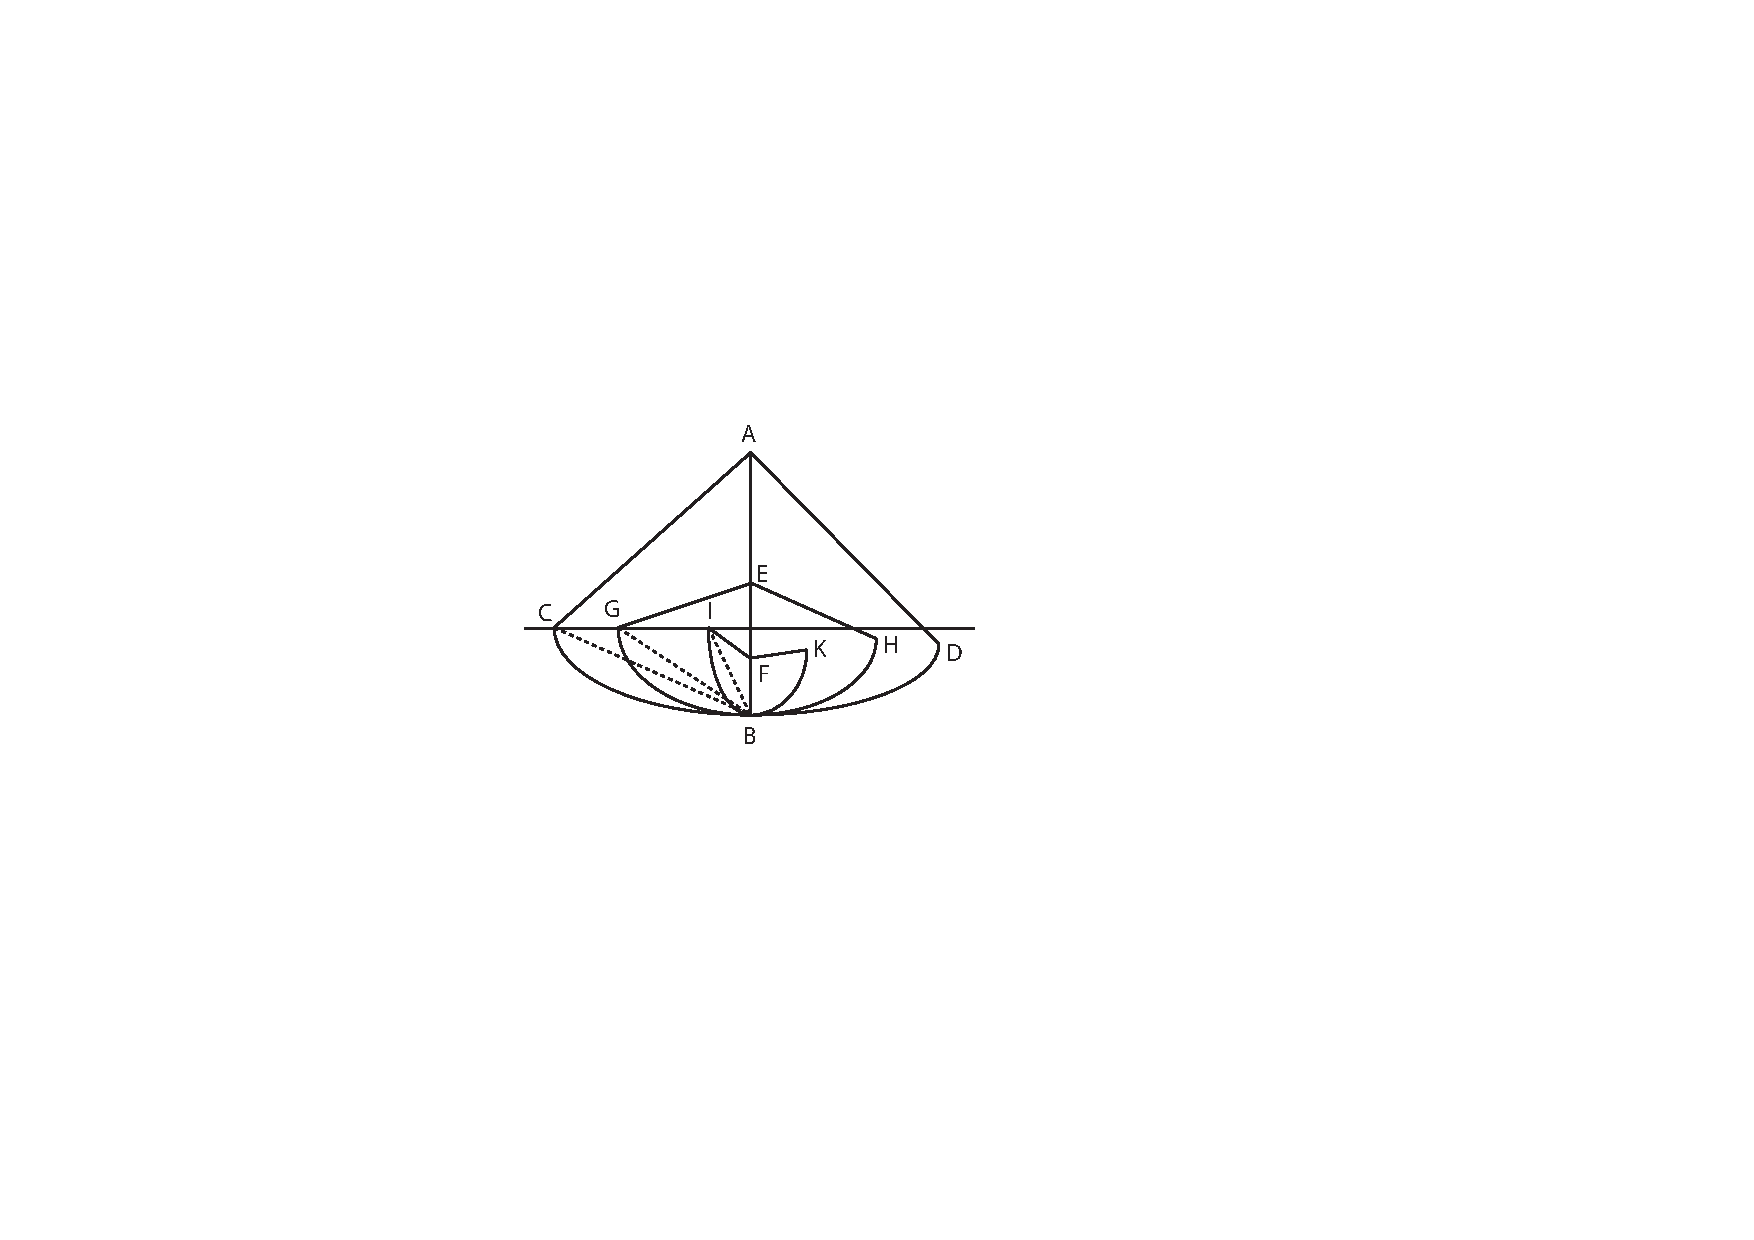
\includegraphics[width=0.55\textwidth]{images/cazreus1645-d2.pdf}\\
\noindent \centering [\textit{Fig. 2}]
\end{center}
%\vspace*{1.0em}%
\pstart%
\noindent%
[p. 12]
[...] neque per diuersos arcus ad eam
\edtext{aequaliter accedunt.
\edtext{Nempe filo pedum quatuor cum dimidio suspensus globus, ad lineam horizontalem,
tribus infra centrum pedibus descriptam, propius quam duobus digitis nunquam accessit.}%
{\lemma{}\Afootnote{\textit{Unterstrichen:}
filo pedum [...] nunquam accessit.}}
At centro nouem tantum digitis supra lineam horizontalem accepto,
filoque duorum pedum constituto, iam globus ad lineam horizontalem,
vno digito quam antea propius accessit.}%
{\lemma{}\Afootnote{\textit{Am Rand markiert:}
Nempe filo pedum [...] antea propius accessit.}}
Vbi vero centrum septem infra lineam horizontalem digitis assumptum est, vix ad quatuor a linea horizontali digitos globus ascendit.
\pend
%\newpage%
\pstart%
\noindent%
[p. 13]
Globus enim per a\"{e}rem semper toto suo pondere deorsum nititur, et eatenus solum eius descensus interturbatur, quatenus a recto et%
\edtext{}{\lemma{}\Afootnote{\textit{Am Rand:}
Imo res eodem redit.}}
perpendiculari cursu, ad circularem cogitur atque adducitur.
\pend 
% \newpage
\count\Afootins=1200
%\vspace*{1.5em}%
\pstart%
\noindent%
[p. 18]
\edtext{Aio igitur, ita esse a natura constitutum, vt globus\protect\index{Sachverzeichnis}{globus} quilibet, cuiuscumque materiae, ex vnius diametri altitudine cadens, duplum sui ponderis\protect\index{Sachverzeichnis}{pondus}, hoc est, praeter pondus\protect\index{Sachverzeichnis}{pondus} quod sine impetu in aequilibrio retineret, aliud sibi aequale attollat; et ex altitudine duarum diametrorum, triplum; ex tribus diametris, quadruplum; et ita deinceps: adeo vt ex quauis altitudine cadens, semper (vltra aequilibrium) toties proprium pondus\protect\index{Sachverzeichnis}{pondus} multiplicatum attollat, quot in tota vnde cadit altitudine diametri continentur.}%
{\lemma{}\Afootnote{\textit{Markierter Absatz.}}}
\pend
\vspace{1em}
\pstart
%%
%\newline\indent%
\noindent[\textit{Neben diesem Absatz folgende gedruckte Marginalie:}]
\pend
\vspace{0.5em}
\pstart
Experientia\protect\index{Sachverzeichnis}{experientia} noua, et admiratione digna, modum, mensuram, ac rationem accelerationis\protect\index{Sachverzeichnis}{acceleratio} motus in naturali grauium descensu euidenter exprimens.
\pend
\vspace{1em}%
\pstart%
\noindent%
[p. 37]
A\"{i}o vero aequalibus temporibus, spatia decurri maiora semper ac maiora in ratione dupla. Diuiso enim spatio \textit{AB}, per quod supponitur fieri descensus, in partes quotcumque aequales, in $C$, $D$, $E$, $F$, etc. iam ostensum est partem secundam $CD$, et primae partis dimidiam partem inferiorem $NC$, aequali tempore percurri, et ob eam quidem causam, quod vt pars $CD$ dupla est partis $NC$, ita velocitas quoque per totam $CD$, dupla sit velocitatis per totam
%%
\edtext{$NC$.}{\lemma{}\Afootnote{\textit{An} totam \textit{NC anschließend:}
Hic incipit Paralogismus,\textsuperscript{[a]}\protect\index{Sachverzeichnis}{paralogimus} duplae sunt anal$\langle$ogiae$,\rangle$\textsuperscript{[b]} singul$\langle$a$\rangle$ singulis, sed non aggregata ag$\langle$gre$\rangle$gatis, quae sunt in quadrupla ratione, seu in duplicata alti$\langle$tu$\rangle$dinum. Et facile intel$\langle$ligi$\rangle$ potest, quod de \textso{duplo} dicit$\langle$ur$\rangle$ esse falsum, nam si semper\textsuperscript{[c]} trisecuis$\langle$set$\rangle$ eodem\textsuperscript{[d]} ratiocinandi modo produxis$\langle$set$\rangle$ \textso{triplum}.%
\vspace*{2mm}\newline\footnotesize%
\textsuperscript{[a]}~Paralogismus, \textit{(1)}\ aequales \textit{(2)}\ duplae \textit{L}
\quad%
\textsuperscript{[b]}~duplae sunt anal$\langle$ogiae,$\rangle$ \textit{erg. L}
\quad%
\textsuperscript{[c]}~semper \textit{erg. L}
\quad%
\textsuperscript{[d]}~eodem \textit{(1)}\ rationandi \textit{(2)}\ ratiocinandi \textit{L}}}
%%
At simili ratione etiam efficitur, velocitatem per totam $DF$, duplam esse velocitatis eius, quae habetur per totam $CD$, sicut tota $DF$, dupla est ipsius $CD$: aequali igitur etiam tempore $CD$, et $DF$, decurruntur: eademque omnino ratio est ipsarum $DF$, et $FK$, caeterarumque omnium se pariter in ratione dupla superantium, vt satis manifestum est: spatia igitur aequalibus temporibus emensa, et velocitates iisdem temporibus aequalibus acquisitae, semper augentur in continua ratione \setline{6}dupla. 
\pend
% \newpage
\vspace{1.0em}%
\pstart%
\centering%
\noindent%
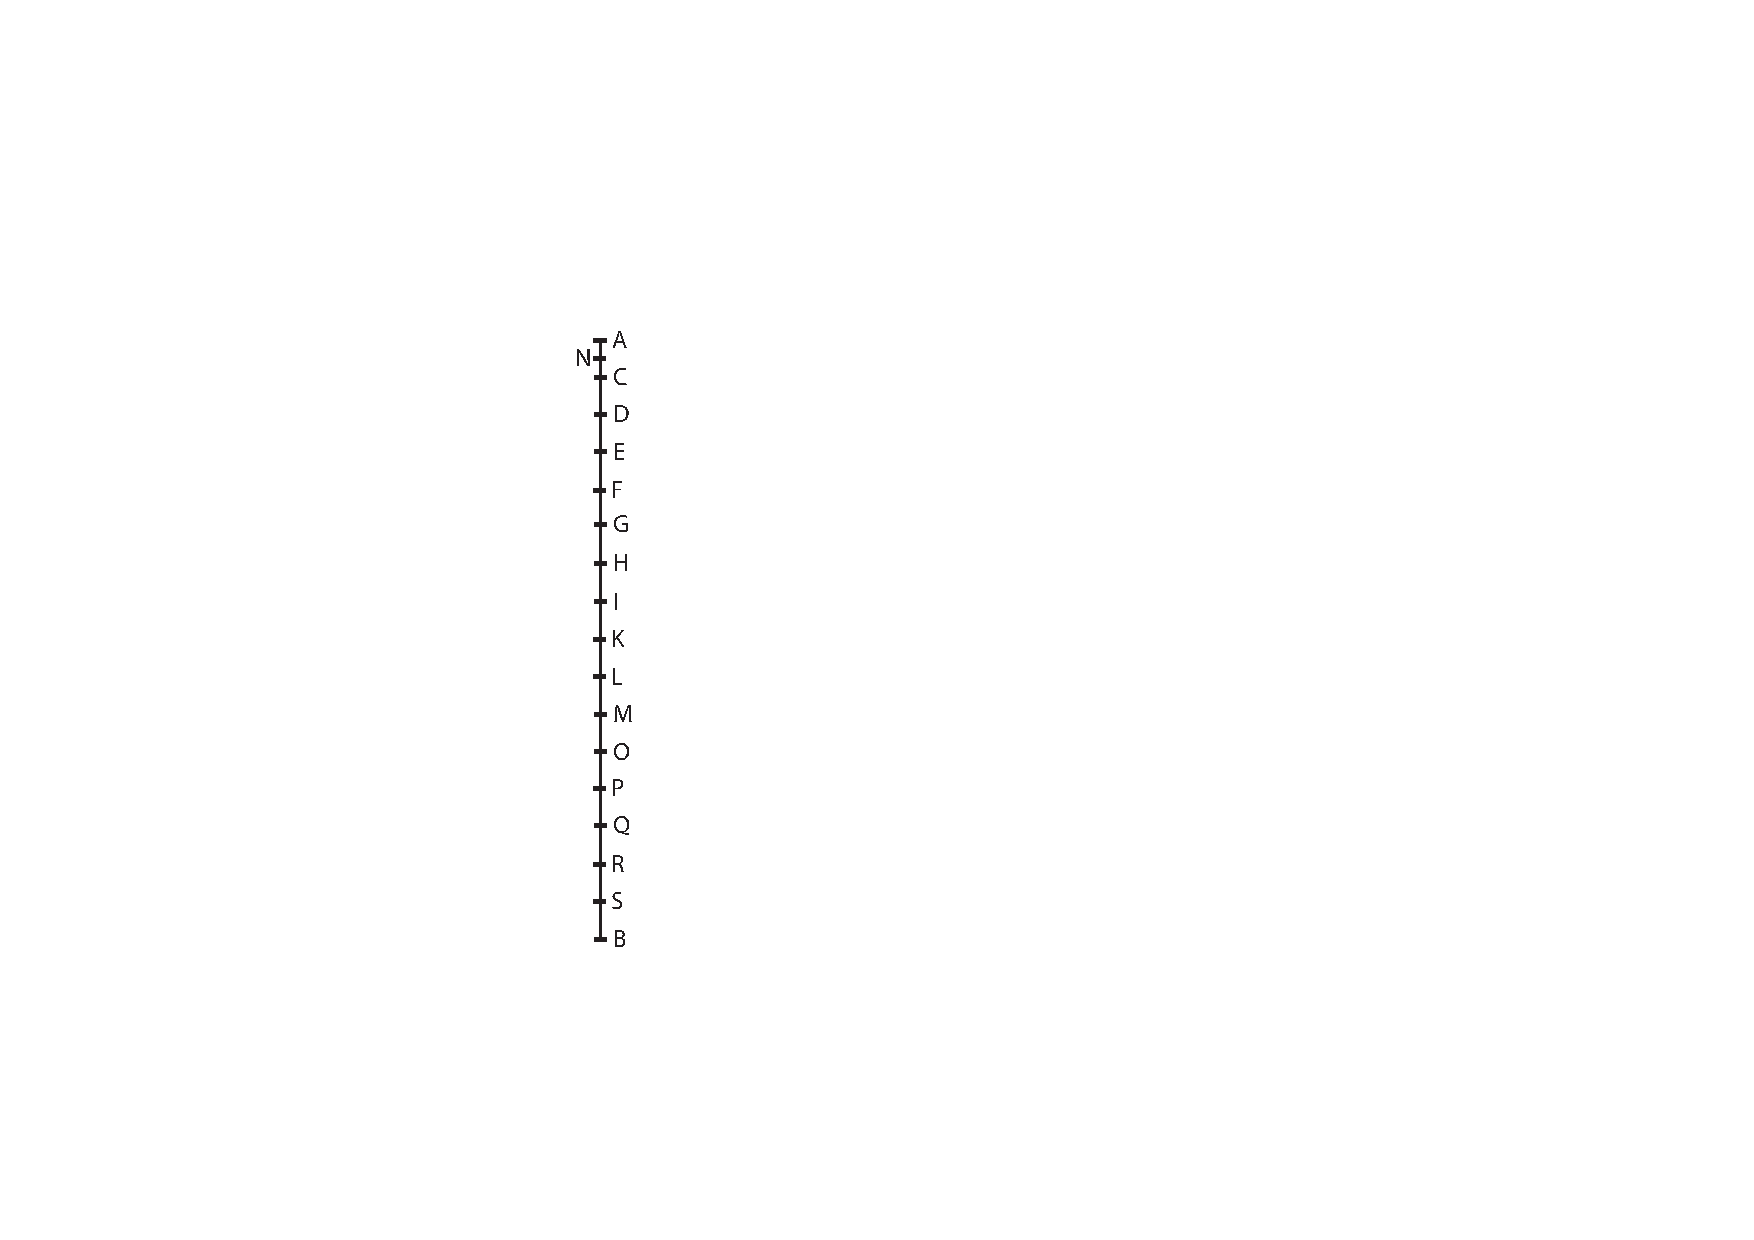
\includegraphics[width=0.08\textwidth]{images/cazreus1645-d3.pdf}%
\pend
%\vspace*{0.5em}%
\pstart%
\centering%
\noindent
[\textit{Fig. 3}] 
\pend
%%%% HIER ENDET DAS STÜCK